\begin{figure}[!ht]
    \centering
    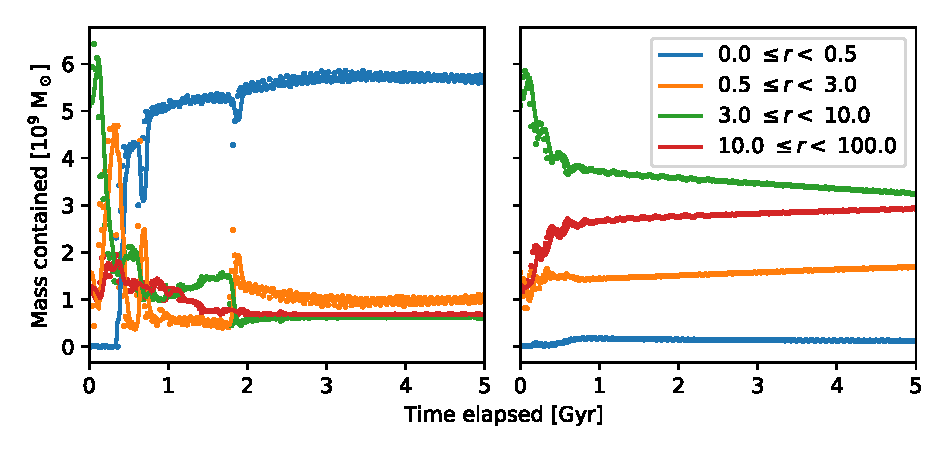
\includegraphics[trim=0 0 0 0.7cm]{sd_r_fig.pdf}
    \caption{The evolution of the (gaseous) mass contained within various shells (see legend) is shown. On the left, the {\tt custom} run is show, with the {\tt default} run being shown on the right. It is clear from this figure that the supernova-driven model causes a large proportion of the gas to be transported into the centre of the galaxy; over 80\% of the gas particles falling into this central region within 1 Gyr of the evolution of the disk. This is unsurprising as the disk was initial highly Toomre-unstable (see the discussion in \S \ref{sec:sigrpred} due to the low pressure support that the {\tt custom} model provides.}
    \label{fig:sd_r_evo}
\end{figure}
Because the initial conditions do not fit the system exactly, there will initially be a significant movement of particles within the disk until it is made marginally Toomre-stable ($Q\approx1$).
For the two models this is shown in Figure \ref{fig:sd_r_evo}.
Due to the fact that the {\tt default} model is more stable at higher surface densities (see Figure \ref{fig:toomreqthr_dat}), there is considerably less mass transport into the centre of the galaxy than with the {\tt custom} model.
The {\tt default} model is also unable to form clumps due to its high pressure support.
This prevents the {\tt default} galaxies from rapidly transporting their mass into the central regions to stabilise the galaxy; it is really the clump formation that drives this process. 

The rapid movement of mass into the central regions highlights three main problems with the simple supernovae-driven model, namely that
\begin{itemize}
    \item The disk is unable to eject mass. Under normal circumstances, supernovae explosions would eject mass vertically back into the IGM.
    \item There is no infall from the IGM at large radii in the galaxy to feed the outer shells.
    \item The stars are only tracers, rather than actually being formed in the simulation, and as such gas cannot be consumed and the gas fraction cannot be lowered.
\end{itemize}
In the {\tt custom} model in particular, this leads to a build-up of mass in the centre of the galaxy which is not seen in nature.
This build-up, which is due to a lack of star-formation prescription, can not be separated from the effects of the model without considerable further work.
The predictions in \S \ref{sec:sigrpred} suggest that whilst there should be a build-up of mass in the centre, it should not be at the $\approx 80\%$ levels that are seen in the {\tt custom} runs.
Those predictions are shown against the simulation data in Figure \ref{fig:toomreqthr_dat}.


\begin{figure}[ht]
    \includegraphics[trim={1.95cm 0cm 1.9cm 1.33cm}]{sd_evo_simulation.pdf}
    \caption{The evolution of the surface density in the {\tt custom} run is shown. Colour encodes $\log\sg$, and is cut off below $0.1 \msun \pc^{-2}$ and above $10^3 \msun \pc^{-2}$ for clarity. Initially the disk violently forms clumps due to the extremely low Toomre $Q$ value. As these clumps are transported to the centre of the galaxy, they are sheared and form a transient spiral structure, whilst enriching the central region of the galaxy with a high volume of gas. In Figure \ref{fig:sd_r_evo} this mass transport is shown in a more quantitative manner. The {\tt custom} run is the only run shown in the interests of space, as all of the {\tt default} runs evolve uniformly and the other {\tt custom} runs in a similar fashion.}
    \label{fig:sd_evo_small}
\end{figure}


The work of \citet{krumholz_is_2016} suggests that it is this transport of mass into the centre of the galaxy that is the stabilising factor, rather than the effective equation of state of the gas.
This work would dispute that; whilst there is mass transport into the centre of the galaxy this is only because in simulations the initial conditions do not fit with the galaxy being marginally stable.
The gas is transported into the centre such that the galaxy can fit the $Q\approx1$ $\sg(r)$ curve which is considerably different from the initial conditions of an exponential disk.
This curve, as shown in \S \ref{sec:sigrpred}, depends on the underlying dark matter structure of the galaxy and the sound speed of the gas.

For an equation of state to be considered valid, it must be able to reproduce the roughly exponential surface density curves that are seen in nature for a typical dark matter profile.
To design such an equation of state, the processes that provide extra pressure to the gas (cosmic rays, magnetic fields, star formation), would allow the galaxy to be marginally stable and yet still reproduce an exponential surface density profile.

